\documentclass[paper=letter,11pt]{scrartcl}

\KOMAoptions{headinclude=true, footinclude=false}
\KOMAoptions{DIV=14, BCOR=5mm}
\KOMAoptions{numbers=noendperiod}
\KOMAoptions{parskip=half}
\addtokomafont{disposition}{\rmfamily}
\addtokomafont{part}{\LARGE}
\addtokomafont{descriptionlabel}{\rmfamily}
%\setkomafont{pageheadfoot}{\normalsize\sffamily}
\setkomafont{pagehead}{\normalsize\rmfamily}
%\setkomafont{publishers}{\normalsize\rmfamily}
\setkomafont{caption}{\normalfont\small}
\setcapindent{0pt}
\deffootnote[1em]{1em}{1em}{\textsuperscript{\thefootnotemark}\ }


\usepackage{amsmath}
\usepackage[varg]{txfonts}
\usepackage[T1]{fontenc}
\usepackage{graphicx}
\usepackage{xcolor}
\usepackage[american]{babel}
% hyperref is needed in many places, so include it here
\usepackage{hyperref}

\usepackage{xspace}
\usepackage{multirow}
\usepackage{float}


\usepackage{braket}
\usepackage{bbm}
\usepackage{relsize}
\usepackage{tcolorbox}

\def\ketY{\ensuremath{\ket {\Psi}}}
\def\iGeV{\ensuremath{\textrm{GeV}^{-1}}}
%\def\mp{\ensuremath{m_{\textrm{proton}}}}
\def\rp{\ensuremath{r_{\textrm{proton}}}}
\def\me{\ensuremath{m_{\textrm{electron}}}}
\def\aG{\ensuremath{\alpha_G}}
\def\rAtom{\ensuremath{r_{\textrm{atom}}}}
\def\rNucl{\ensuremath{r_{\textrm{nucleus}}}}
\def\GN{\ensuremath{\textrm{G}_\textrm{N}}}
\def\ketX{\ensuremath{\ket{\vec{x}}}}
\def\ve{\ensuremath{\vec{\epsilon}}}


\def\ABCDMatrix{\ensuremath{\begin{pmatrix} A &  B  \\ C  & D \end{pmatrix}}}
\def\xyprime{\ensuremath{\begin{pmatrix} x' \\ y' \end{pmatrix}}}
\def\xyprimeT{\ensuremath{\begin{pmatrix} x' &  y' \end{pmatrix}}}
\def\xy{\ensuremath{\begin{pmatrix} x \\ y \end{pmatrix}}}
\def\xyT{\ensuremath{\begin{pmatrix} x & y \end{pmatrix}}}

\def\IMatrix{\ensuremath{\begin{pmatrix} 0 &  1  \\ -1  & 0 \end{pmatrix}}}
\def\IBoostMatrix{\ensuremath{\begin{pmatrix} 0 &  1  \\ 1  & 0 \end{pmatrix}}}
\def\JThree{\ensuremath{\begin{pmatrix}    0 & -i & 0  \\ i & 0  & 0 \\ 0 & 0 & 0 \end{pmatrix}}} 
\def\JTwo{\ensuremath{\begin{bmatrix}    0 & 0 & -i  \\ 0 & 0  & 0 \\ i & 0 & 0 \end{bmatrix}}}
\def\JOne{\ensuremath{\begin{bmatrix}    0 & 0 & 0  \\ 0 & 0  & -i \\ 0 & i & 0 \end{bmatrix}}}
\def\etamn{\ensuremath{\eta_{\mu\nu}}}
\def\Lmn{\ensuremath{\Lambda^\mu_\nu}}
\def\dmn{\ensuremath{\delta^\mu_\nu}}
\def\wmn{\ensuremath{\omega^\mu_\nu}}
\def\be{\begin{equation*}}
\def\ee{\end{equation*}}
\def\bea{\begin{eqnarray*}}
\def\eea{\end{eqnarray*}}
\def\bi{\begin{itemize}}
\def\ei{\end{itemize}}
\def\fmn{\ensuremath{F_{\mu\nu}}}
\def\fMN{\ensuremath{F^{\mu\nu}}}
\def\bc{\begin{center}}
\def\ec{\end{center}}
\def\nus{$\nu$s}

\def\adagger{\ensuremath{a_{p\sigma}^\dagger}}
\def\lineacross{\noindent\rule{\textwidth}{1pt}}

\newcommand{\multiline}[1] {
\begin{tabular} {|l}
#1
\end{tabular}
}

\newcommand{\multilineNoLine}[1] {
\begin{tabular} {l}
#1
\end{tabular}
}



\newcommand{\lineTwo}[2] {
\begin{tabular} {|l}
#1 \\
#2
\end{tabular}
}

\newcommand{\rmt}[1] {
\textrm{#1}
}


%
% Units
%
\def\m{\ensuremath{\rmt{m}}}
\def\GeV{\ensuremath{\rmt{GeV}}}
\def\pt{\ensuremath{p_\rmt{T}}}


\def\parity{\ensuremath{\mathcal{P}}}

\usepackage{cancel}
\usepackage{ mathrsfs }
\def\bigL{\ensuremath{\mathscr{L}}}

\usepackage{ dsfont }



\usepackage{fancyhdr}
\fancyhf{}


\lhead{\Large 33-444} % \hfill Introduction to Particle Physics \hfill Spring 2020}
\chead{\Large Introduction to Particle Physics} % \hfill Spring 2020}
\rhead{\Large Spring 2020} % \hfill Introduction to Particle Physics \hfill Spring 2020}

\begin{document}
\thispagestyle{fancy}

\begin{center}
{\huge \textbf{Lecture 24}}
\end{center}

{\fontsize{14}{16}\selectfont

\bc
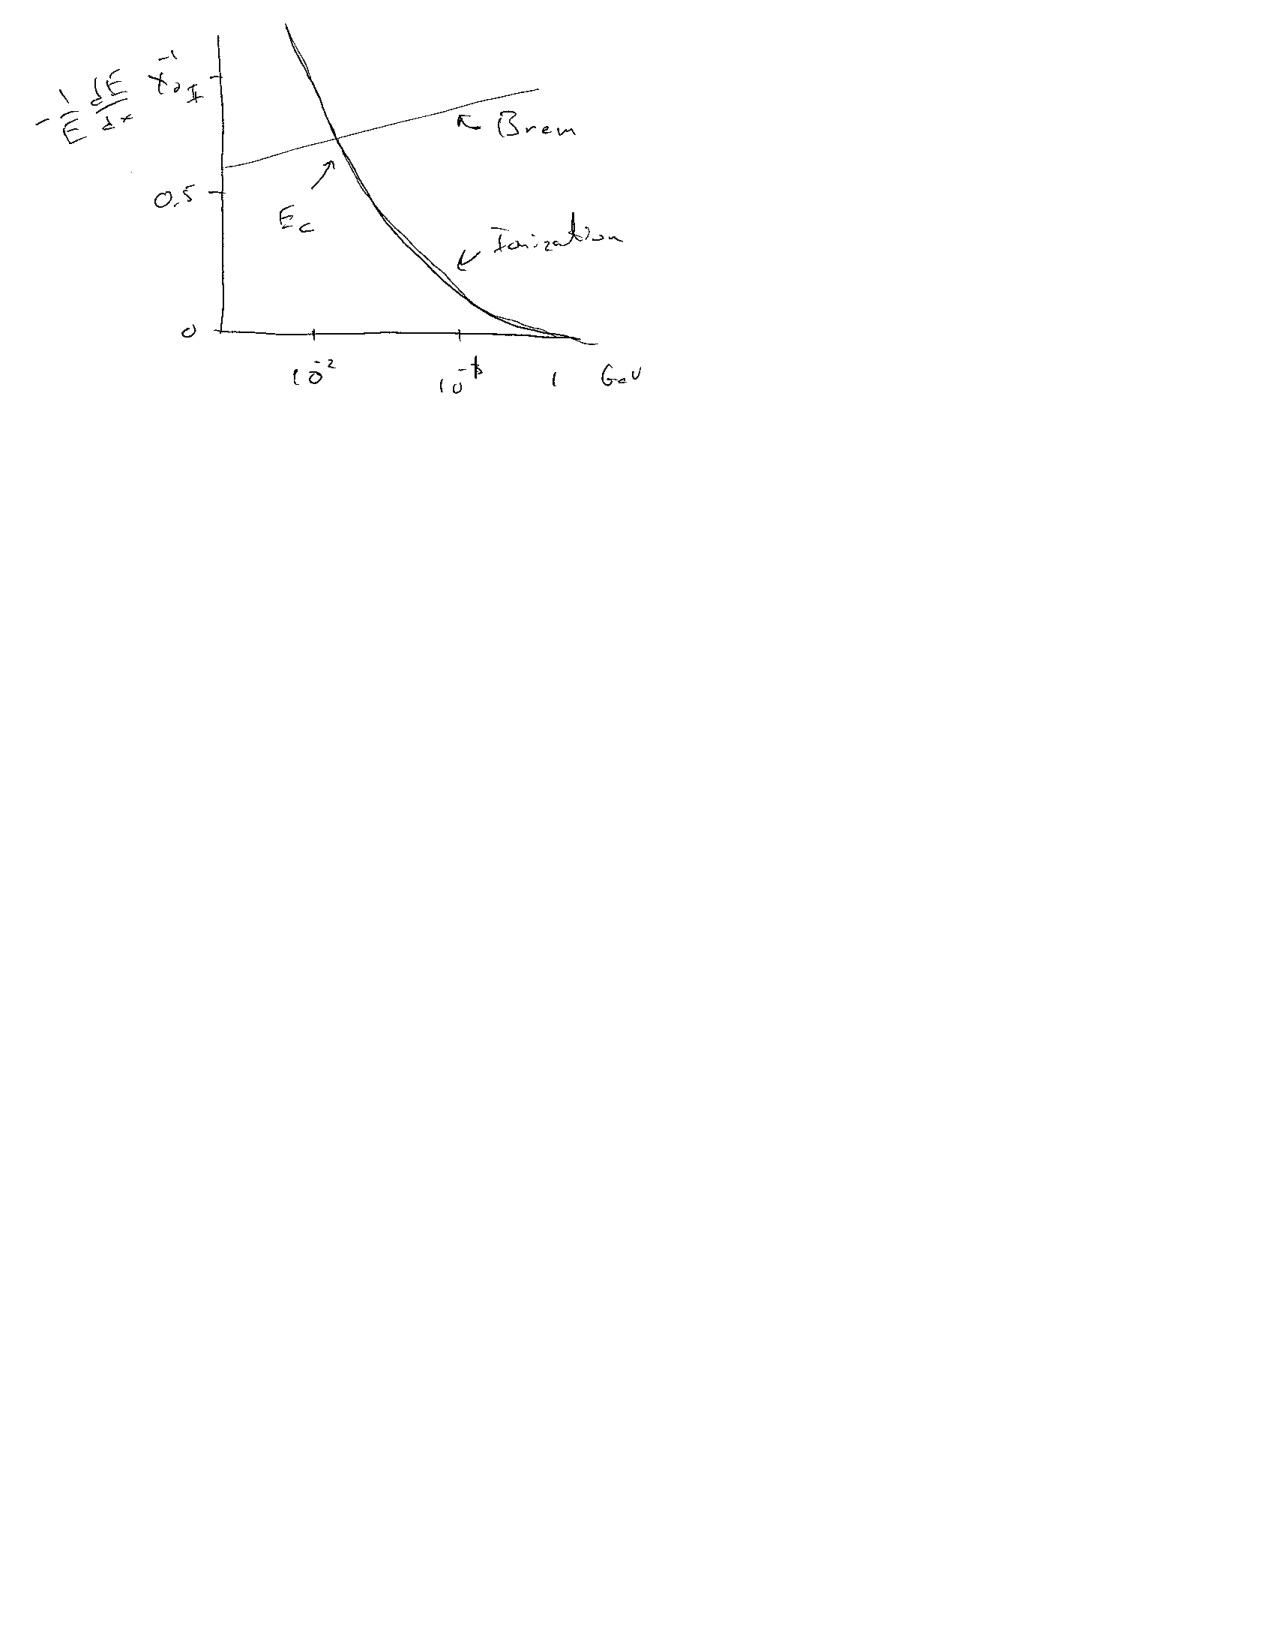
\includegraphics[width=0.8\textwidth]{./DeDxRadiation.pdf}
\ec

Similar story for photons. 

$E_c$ - critical energy O($10^{-2} - 10^{-1}$ GeV)

\begin{minipage}{0.5\textwidth}
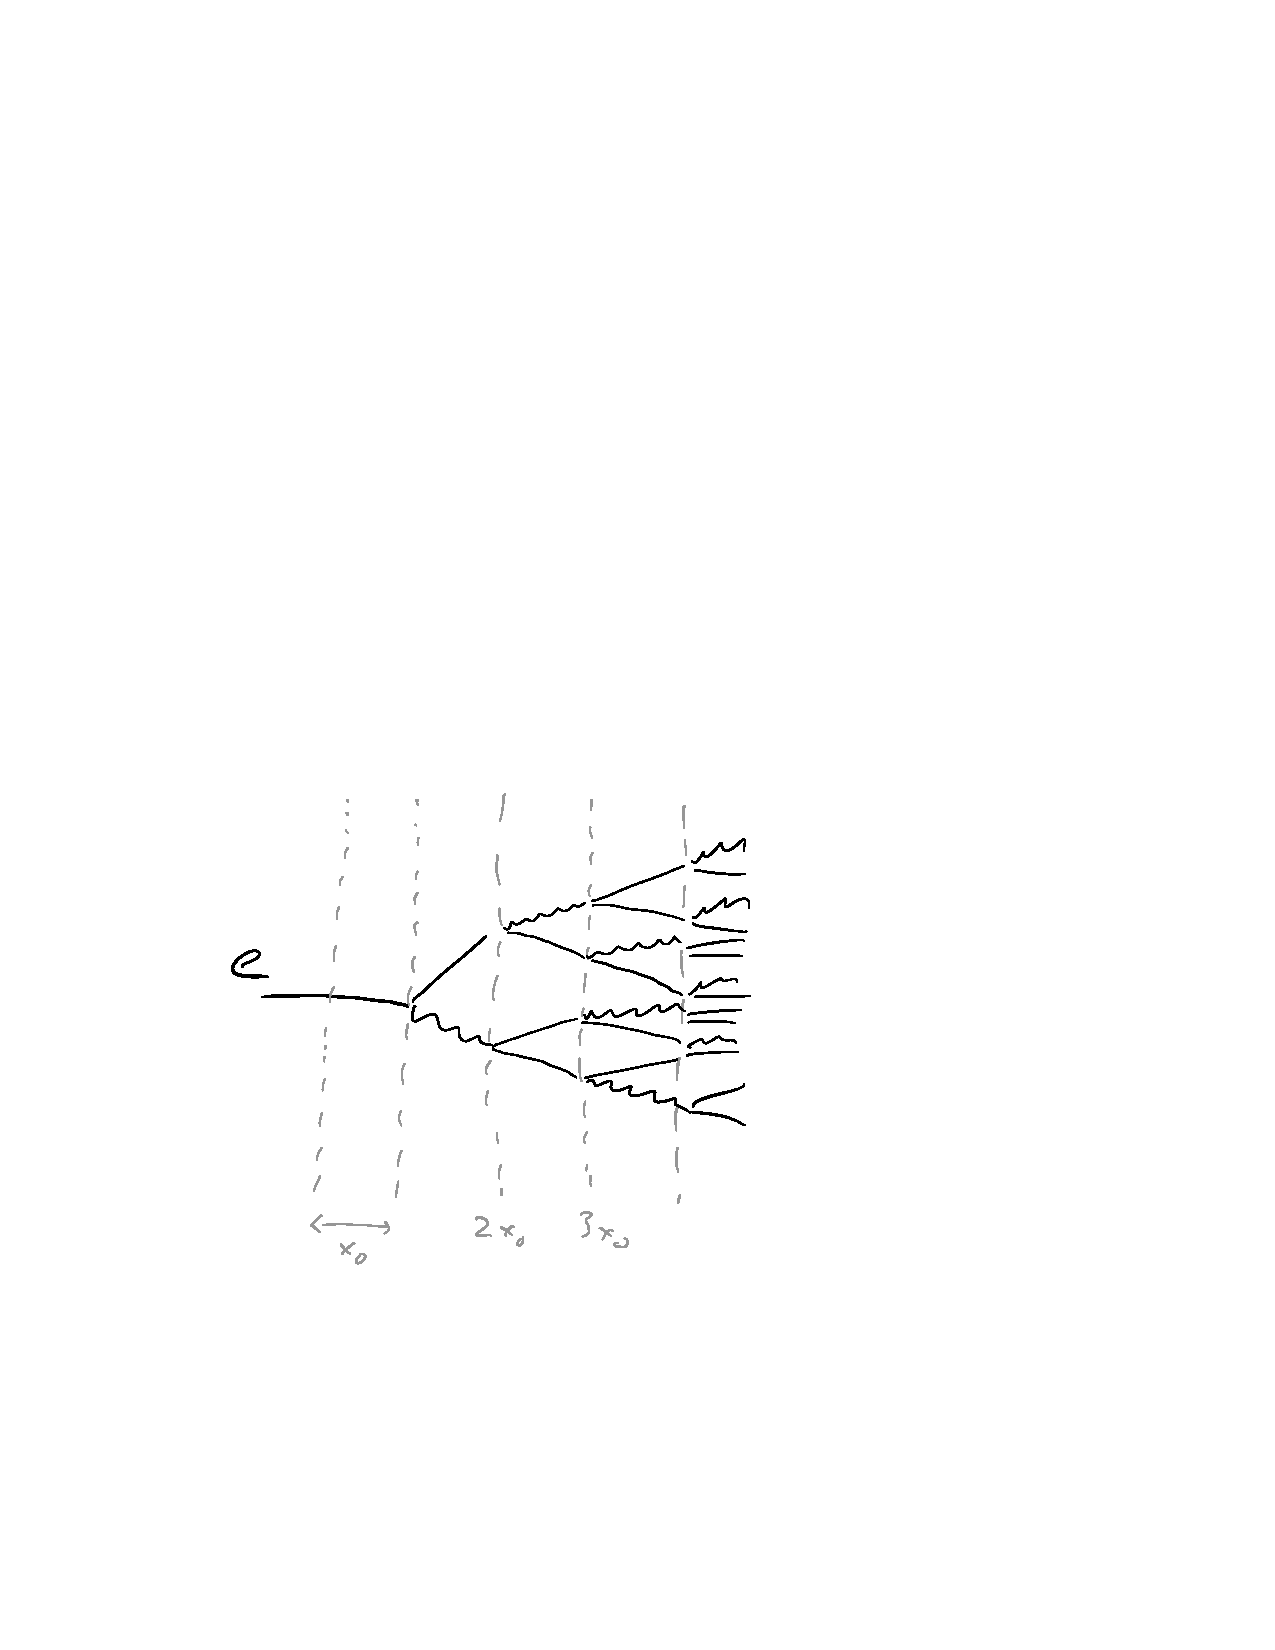
\includegraphics[width=0.8\textwidth]{./ElectronShower.pdf}
\bc
Looks Similar to 
\ec
\includegraphics[width=0.8\textwidth]{./PhotonShower.pdf}
\end{minipage}\hfill
\begin{minipage}{0.5\textwidth}
\bc
\textbf{``Electromagnetic Shower''}
\ec

-) For each e (or $\gamma$) with $E > E_c$ travels $\sim 1 x_0$ then gives up 1/2 energy to $\gamma$ (or ee).\\

-) e's, $\gamma$'s with energy $< E_c$ get absorbed via ionization\\

If initial energy $E_0 >> E_c$ then after t-radiation lengths there will be $2^t$ particles. 
Approximately equal e's and $\gamma$'s each with energy $E(t) \sim \frac{E_0 }{2^t}$.

\end{minipage} 

Shower will stop growing when 
\be
E(t) \simeq E_c \equiv E(t_{max})
\ee
$t_{max}$ is point in shower with max particles

\be
t_{max} = \frac{\ln \frac{E_0}{E_c}}{\ln 2}
\ee

$\Rightarrow$ shower depth grows as $\ln$

$N_{max}$ given by $E_0/E_c$

\lineacross\\
For heavier particles, Brem does not kick in until much higher energies.
eg: $    E_c \sim 3000$ GeV for a muon in lead.

\clearpage


\underline{\textbf{Nuclear Interactions} }

If the particle traversing the medium is a hadron, can interact via the strong interaction.

eg: $\pi^\pm$ moving through detector material will suffer an inelastic collision in distance $\lambda_i$

This collision takes energy from $\pi$ and converts it to additional hadrons (charged and neutral)

Leads to what is called ``Hadronic Shower'' - same basic idea as an EM shower, but much more complex.
Involves a variety of processes at different length scales

\bc
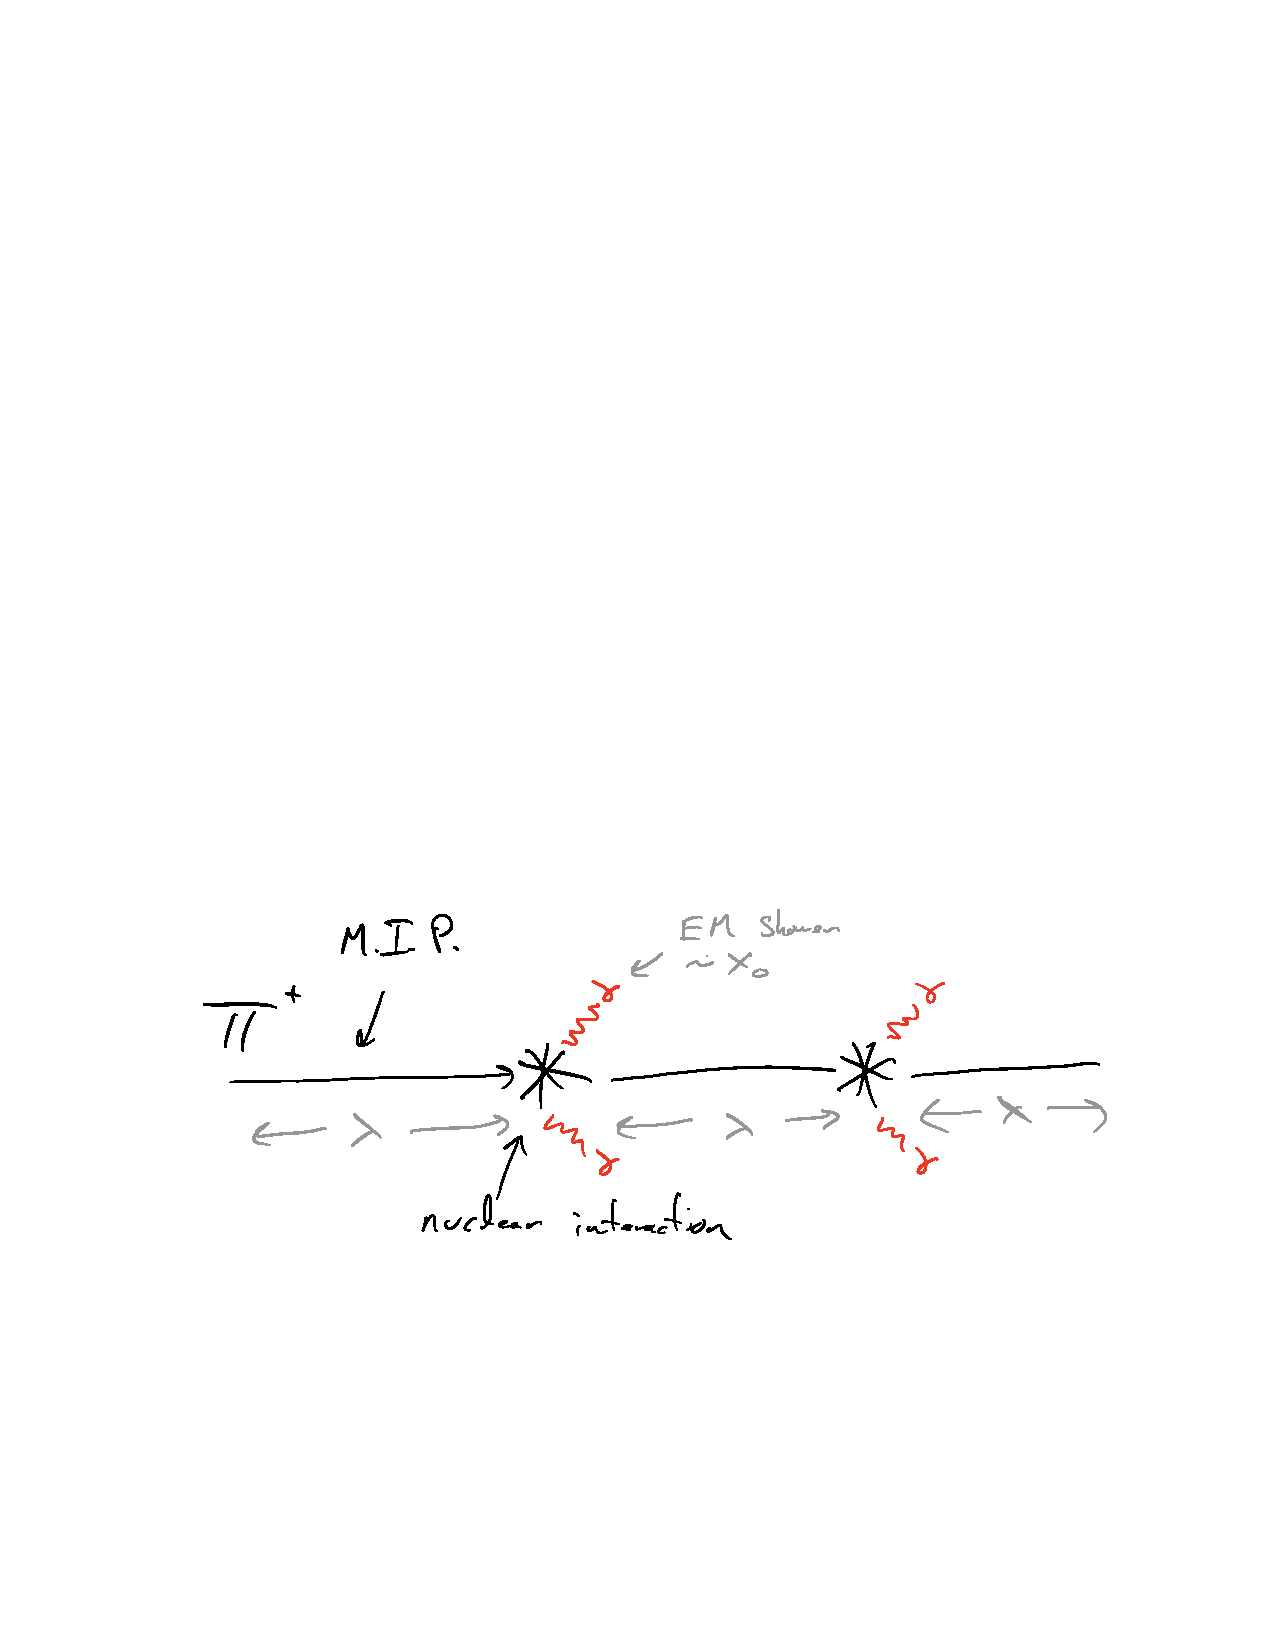
\includegraphics[width=0.8\textwidth]{./hadronicShowerNew.pdf}
\ec

At the inelastic collision, typically produce 
\bi
\item[$\pi^+$] $\sim 1/3$ of the time. Travels like a MIP w/scale $\lambda_i$
\item[$\pi^0$] $\sim 1/3 \leftarrow Br(\gamma\gamma) \sim 100\%\ \rmt{travels 10nm} \Rightarrow $ EM shower w/ scale $X_0$
\item[$\pi^-$] $\sim 1/3$ 
\ei

Both $\pi^\pm$ travel like MIPs of order $\lambda_i$.
$\Rightarrow$ Hadronic showers develop over larger distances and contain much more fluctuations.

\lineacross

\clearpage

\textbf{\underline{Trackers}}

Ionization detectors in a magnetic field.

Charged particles traveling in a magnetic field move in circles. 

\be
\frac{1}{R[\m]} = Q \cdot B[T] \cdot \frac{0.3}{p_T[\GeV]}
\ee

Particle positions are measured by finely etched silicon sensors.\\
$\sim10 \mu\m$ resolution

We measure the curvature $\sim \frac{1}{R} \sim \frac{1}{\pt}$

\begin{minipage}{0.3\textwidth}
\bc
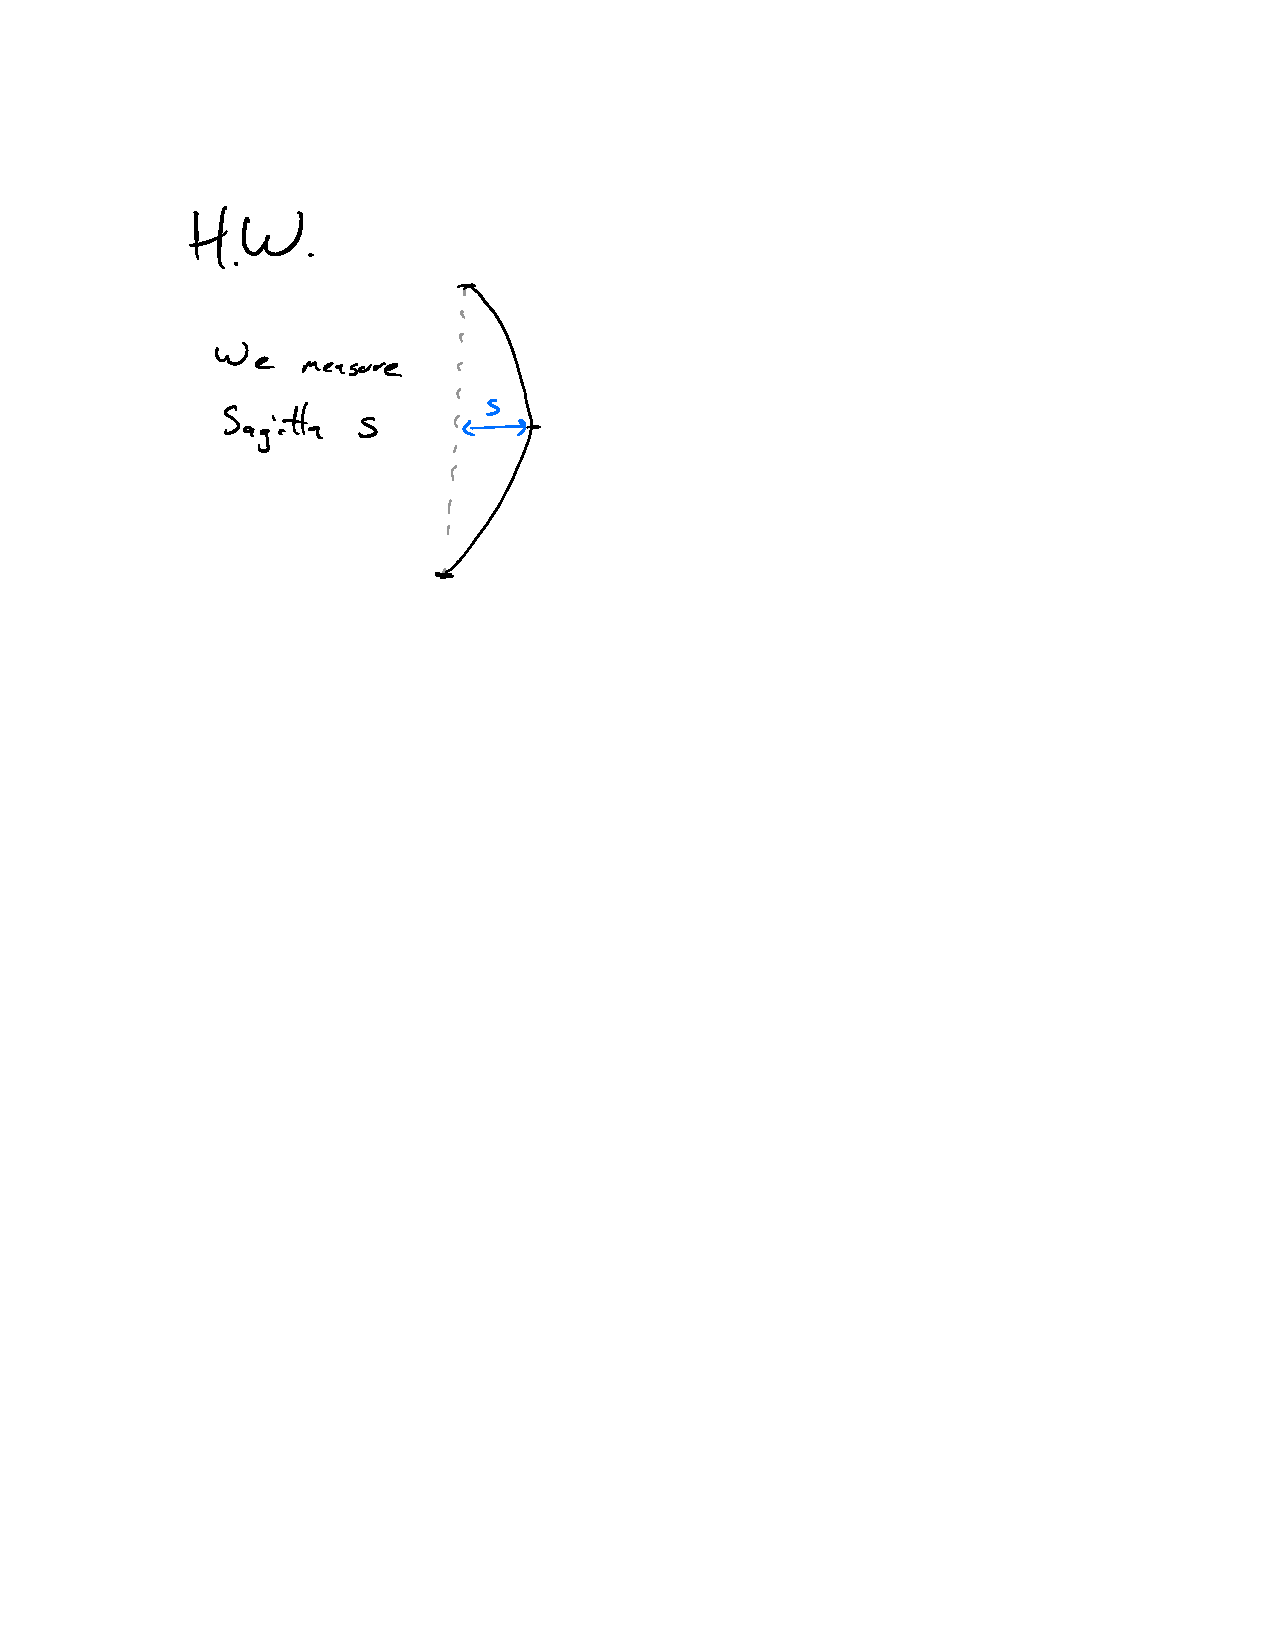
\includegraphics[width=0.9\textwidth]{./sagittaNew.pdf}
\ec
\end{minipage}\hfill
\begin{minipage}{0.7\textwidth}
\be
s  = \frac{qBL^2}{8\pt}
\ee
(More important to have bigger length than larger B)

\be
\Rightarrow \Delta \frac{1}{\pt} = \frac{\Delta \pt }{\pt^2}
\ee

So the relative uncertainty in \pt\ degrades with \pt.
\end{minipage}

\underline{LHC} typical performance

\be
\frac{\Delta \pt}{\pt} \sim (\rmt{few \%}) \frac{\pt}{100\ \GeV}
\ee

\clearpage
\textbf{\underline{EM Calorimeter}}

Contains and measures e's $\gamma$'s and $\pi^0\rightarrow\gamma\gamma$.
\bc
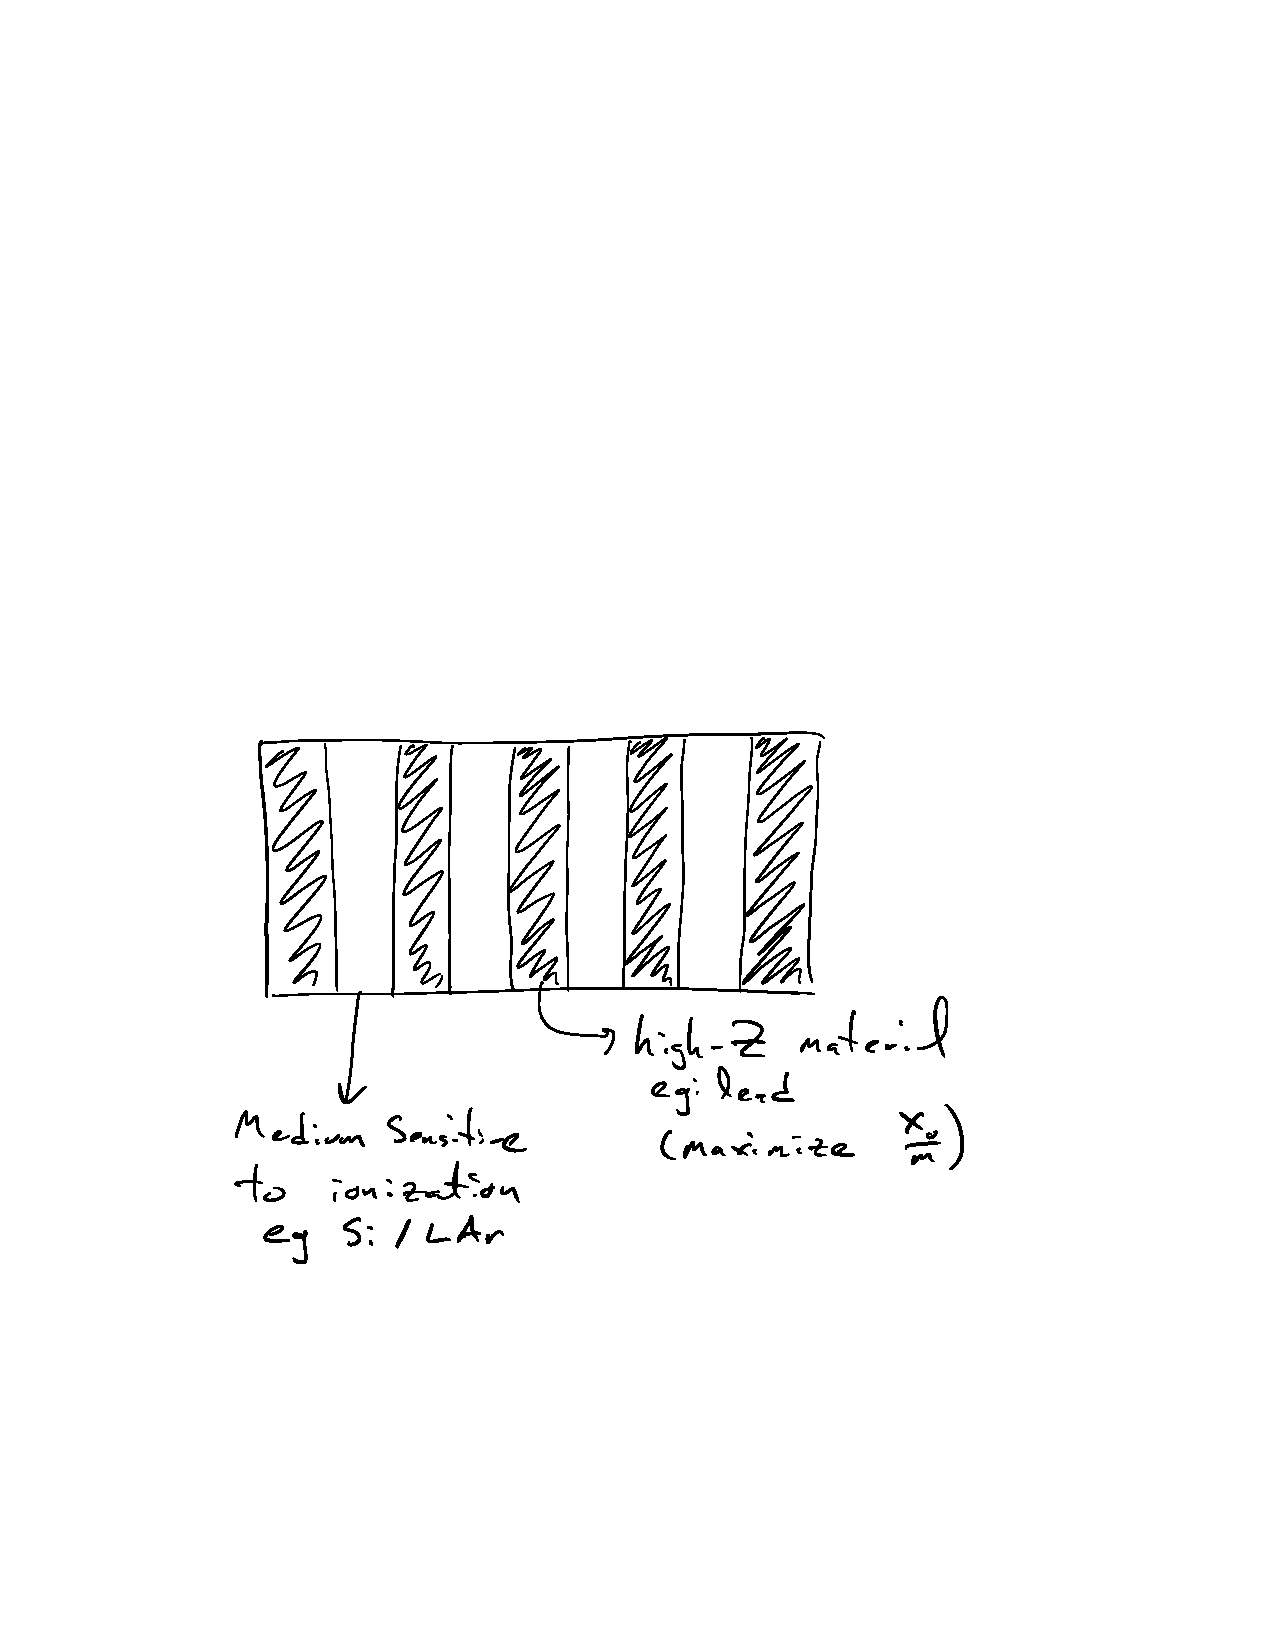
\includegraphics[width=0.5\textwidth]{./EMCalorimeterNew.pdf}
\ec
Total depth $\sim 20 X_0$ (Enough to contain high \pt\ showers)

\begin{minipage}{0.3\textwidth}
\bc
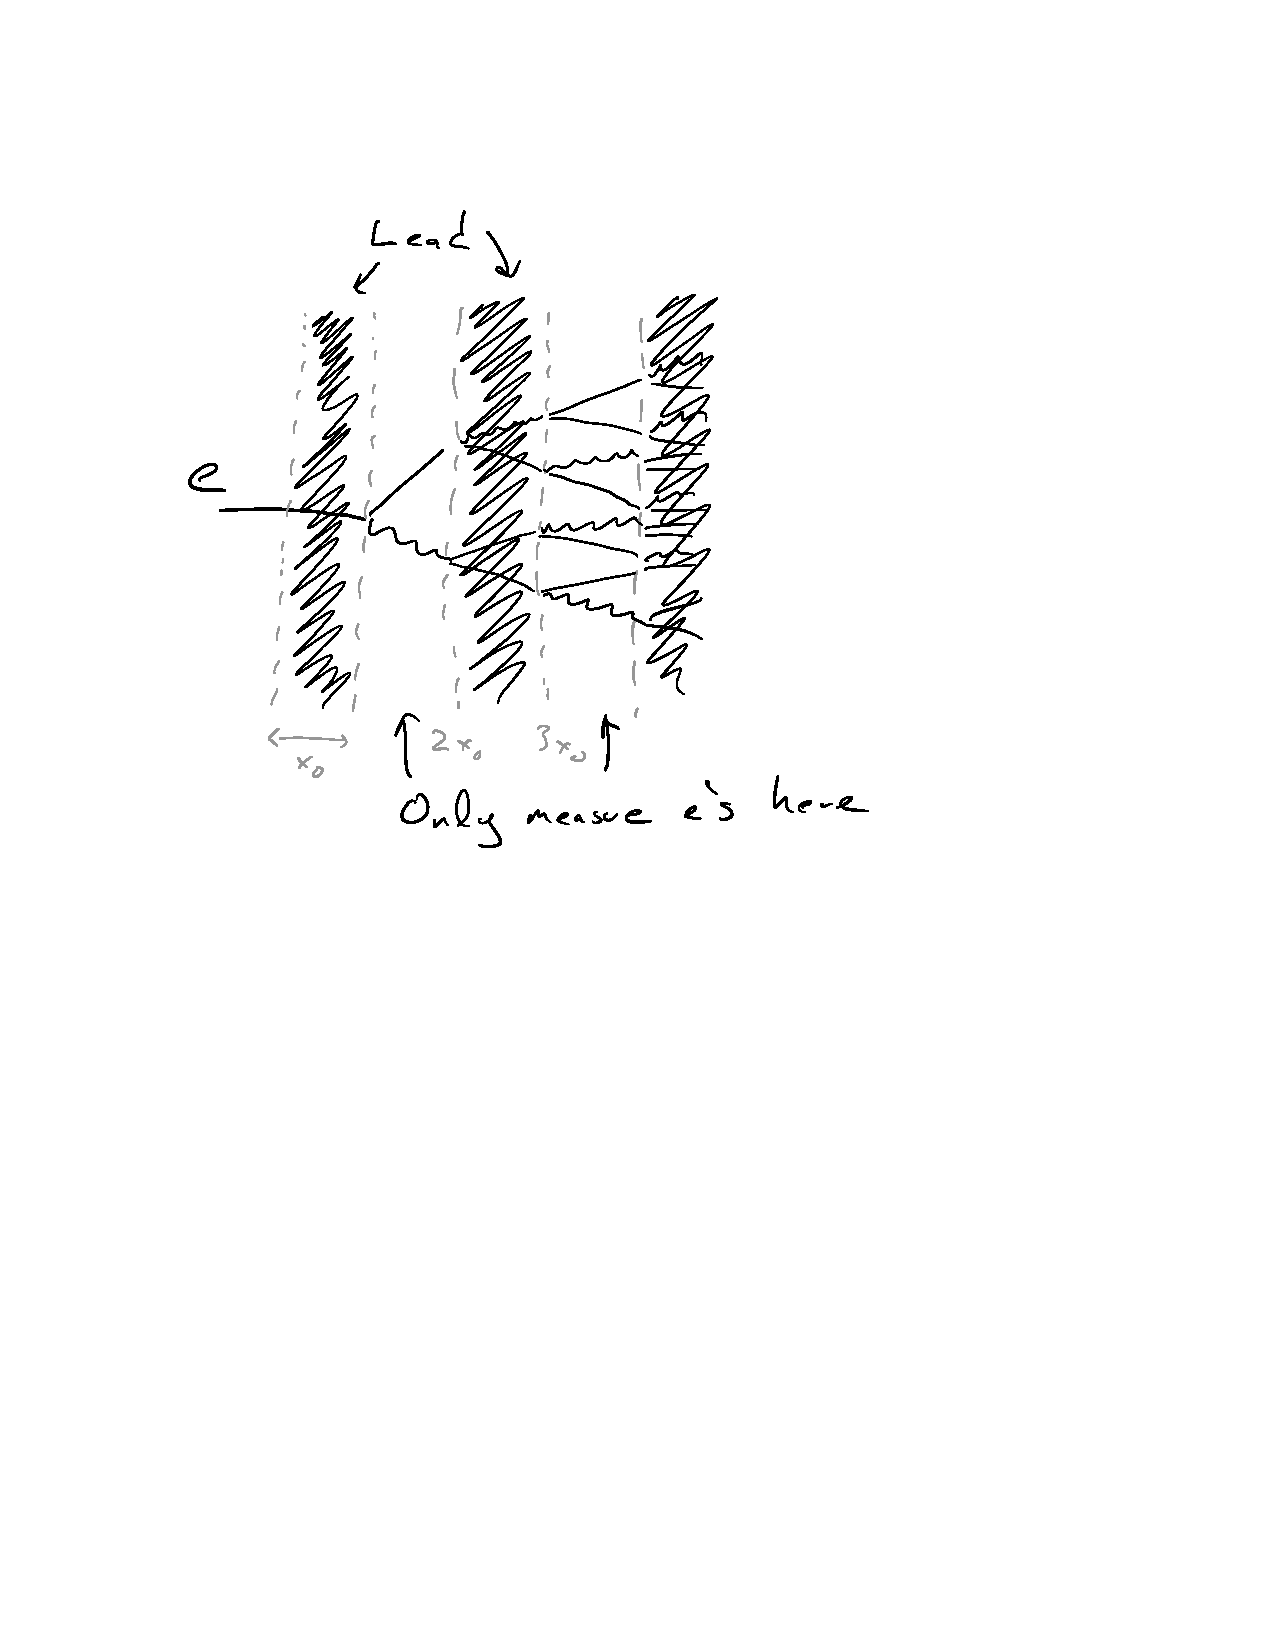
\includegraphics[width=0.9\textwidth]{./EMReadout.pdf}
\ec
\end{minipage}\hfill
\begin{minipage}{0.7\textwidth}
Only energy deposited in Si/LAr  is measured. 

Rest is lost in uninstrumented lead.
\end{minipage}

So only a small fraction of the total EM shower energy is collected (measured).

$E \sim N_c$ amount collected scales like the number of electrons produced

\be
\frac{\Delta E}{E} \sim \frac{\Delta N_c}{N_c} \sim \frac{1}{\sqrt{N_c}} \sim \frac{1}{\sqrt{E}}
\ee

At the LHC typical performance

\be
\frac{\Delta E}{E} \sim  \frac{10\ \%}{\sqrt{E}}
\ee

Unlike trackers the relative energy measurement improves with E.

\clearpage
\textbf{\underline{Hadronic Calorimeter}}

Compare shooting a $\pi^\pm$ in the detector instead of an electron.

\bi
\item[-]$\pi$ will travel further because it has to interact via the strong force (shorted range than EM)
\item[-]$\pi$ will make other $\pi^\pm$ and $\pi^0$
\item[-]Compared to electrons, make less particles (fewer at fixed E) b/c $\pi$ mass is bigger.
\item[-]More varied showers depending on what particles are produced $\pi^\pm$ vs $\pi^0$.
\ei

$\Rightarrow$ hadronic calorimeters need to be bigger, and will measure showers that have more fluctuations.

At the LHC typical performance worse than for EM calorimeters

\be
\frac{\Delta E}{E} \sim  \frac{50\ \%}{\sqrt{E}}
\ee

Relative energy measurement also improves with E.


\textbf{\underline{Muon Detectors}}

Put tracking detectors outside of the calorimeters. 

If any charged particle makes it through $\sim3\m$ of lead it has to be a muon. 

$\mu$ \multiline{no strong interaction \\ only rarely radiate $\gamma$s (below $\sim 3$ TeV)}

\textbf{\underline{Neutrino Detectors at the LHC}}

$\nu$s leave no energy in detector.  

Can infer their presence from momentum imbalance in the transverse plane.

Poor resolutions, b/c have to measure everything else in the event.

\textbf{\underline{Trigger}}

LHC provides bunch crossings at 40 MHz and each event is $\sim 2$KB.

 $\Rightarrow $ 80 Tb/s 

Library of Congress is $\sim 10$ Tb

Can only afford to keep 2 GB/s

Only keep 1 out of 40,000 events.

(Will talk about this more in the next lecture)


}
\end{document}


